\documentclass{article}

\usepackage{graphicx}
\usepackage{textpos}
\usepackage{hyperref}
\usepackage{xcolor}
\usepackage{enumitem}

\setitemize[1]{leftmargin=0ex,labelsep=10pt}

\newcommand\hsep{ {\color{gray}/} }
\newcommand\partitle[1]{\vskip20pt\par\noindent{\textsf{\textbf{#1}}}}

\usepackage{fontawesome}

\begin{document}

\begin{textblock}{2}(8,0)
    \noindent
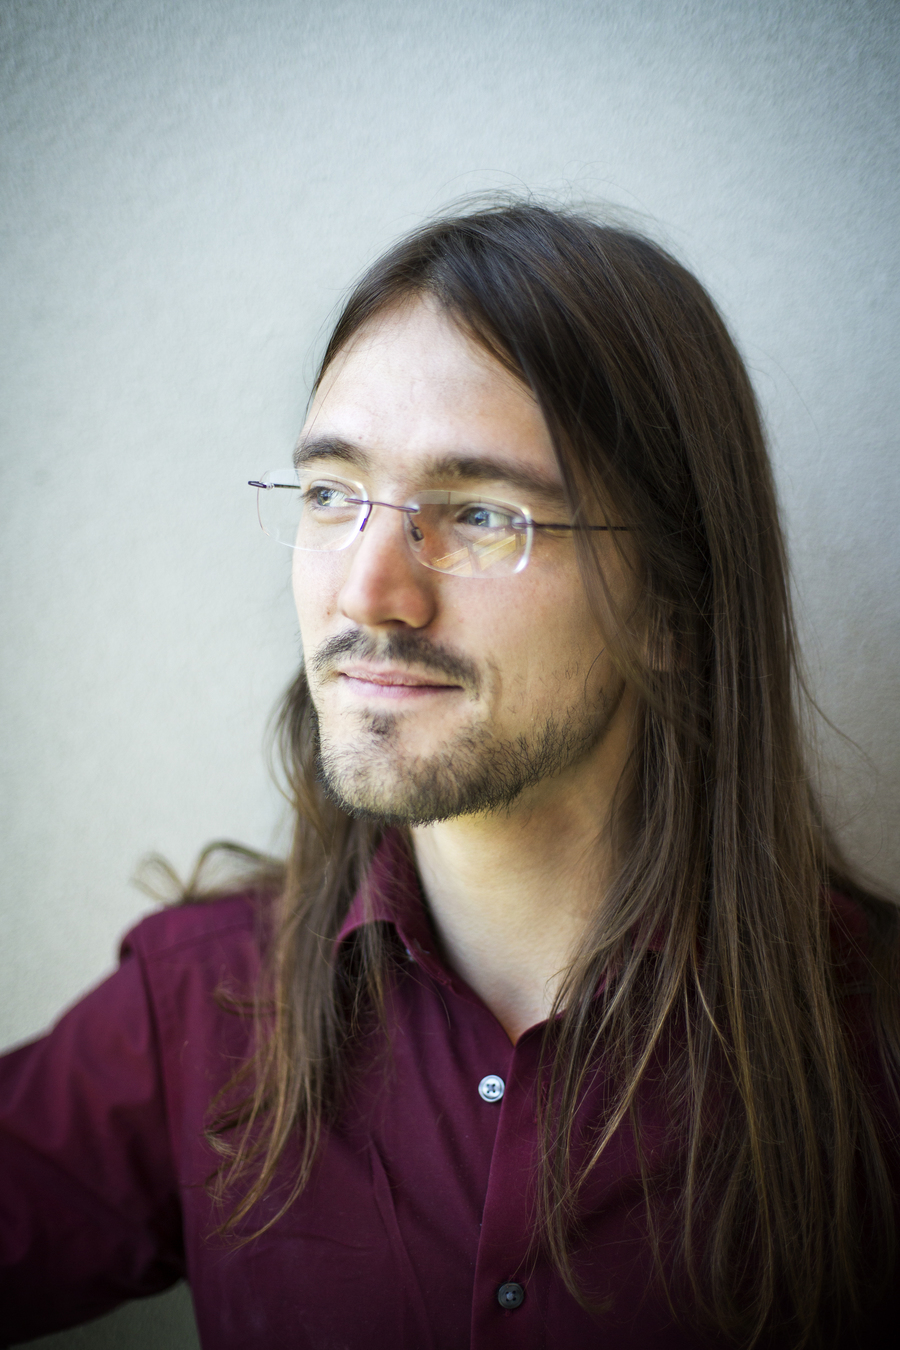
\includegraphics[width=\textwidth]{me}
        \footnotesize(2019)
\end{textblock}\noindent
\textsf{\Large dr.~Bas Westerbaan}\\
academic curriculum vitae December~2020\\

\noindent
\href{mailto:bas@westerbaan.name}{\faEnvelopeO\ bas@westerbaan.name} \hsep
\href{https://bas.westerbaan.name}{\faExternalLink\ bas.westerbaan.name}\\
\href{https://scholar.google.nl/citations?user=AN7BEa8AAAAJ}{%
    \faGraduationCap\ Google Scholar}
    \hsep \href{https://github.com/bwesterb}{\faGithub\ \texttt{bwesterb}}
    \hsep \href{https://www.linkedin.com/in/baswesterbaan/}{\faLinkedinSquare} \\
$*$ 1988, the Netherlands

\partitle{Academic career}
\begin{itemize}
    \item[2020] \emph{Post-doctoral researcher} --- Radboud Universiteit
    \item[februari 2020] \emph{Research visit to
        \href{https://www.ioc.ee/~pawel/}{prof.~dr.~Pawel Sobocinski}}
            at \href{https://www.taltech.ee}{Taltech}.
    \item[2019 -- 2020] \emph{Research fellow} (0.2fte) --- 
        \href{https://cloudflare.com}{Cloudflare} \\
        At the cryptography group of Nick Sullivan.
    \item[2019 -- 2020] \emph{Post-doctoral researcher} (1fte) --- University
        College London\\
        At the \href{http://pplv.cs.ucl.ac.uk/welcome/}{PPLV group}
            under \href{https://alexandrasilva.org/#/main.html}{prof.~dr.~Silva}.
    \item[2018 -- 2019] \emph{Post-doctoral researcher} --- Radboud Universiteit\\
        On the \href{https://pep.cs.ru.nl}{Polymorphic Encryption and Pseudonymisation (PEP) project}.
    \item[april 2018] \emph{Research visit to \href{http://www.cs.ox.ac.uk/people/samuel.staton/main.html}{prof.~dr.~Staton} at Oxford University}
    \item[march 2018] \emph{Invited speaker \href{http://homepages.inf.ed.ac.uk/cheunen/cvqt/}{Combining Viewpoints in Quantum Theory}}\\
        At The University of Edinburgh.
    \item[2013 -- 2018]  \emph{Promovendus (Ph.D-student) ---
        Radboud Universiteit}\\
        At the \href{http://www.ru.nl/ds/}{Digital Security group}
        of Radboud University funded by
        the ERC Advanced Grant \href{https://cordis.europa.eu/project/rcn/107285_en.html}{`Quantum Logic, Computation and Security'}
        of \href{http://www.cs.ru.nl/B.Jacobs/}{prof.~dr.~Bart Jacobs}.
            Defended
            \href{http://westerbaan.name/~bas/thesis.pdf}{thesis}
            on May 14th, 2019.
    \item[2016] \emph{Research visit \href{http://manoa.hawaii.edu}{University of Hawai'i}}\\
        2 month visit to group of \href{http://dusko.org}{prof.~dr.~Pavlovic}
    \item[2007 -- 2013] \emph{B.Sc \& M.Sc degrees in Mathematics ---
                Radboud Universiteit} \\
        M.Sc thesis \href{www.ru.nl/publish/pages/813276/masterscriptie_bas_westerbaan.pdf}{`Sequential Product on Effect Logics'}
            supervised by \href{http://www.cs.ru.nl/B.Jacobs/}{prof.~dr.~Jacobs} \hsep
        B.Sc thesis \href{https://arxiv.org/abs/1409.1030}{`On Effective Undecidability and Post's Problem'}
            supervised by \href{http://www.ru.nl/wiskunde/@1039532/veldman-dhr-dr-(wim)/}{dr.~Veldman}.
        The Master degree was awarded \emph{cum laude}.
\end{itemize}

\partitle{Selected publications}
\begin{itemize}
    \item[2020] \emph{\href{https://sphincs.org/data/sphincs+-round3-specification.pdf}{SPHINCS$^+$ ---
        submission to the 3\textsuperscript{rd} round of the NIST post-quantum project}}\\
    {\footnotesize Aumasson, Bernstein, Beullens, Dobraunig, Eichlseder, Fluhrer,
        Gazdag, H\"ulsing, Kampanakis, K\"olbl, Lange, Lauridsen, Mendel,
        Niederhagen, Rechberger, Rijneveld, Schwabe, BW}\\
    We propose a post-quantum stateless hash-based signature scheme
            with a security reduction to 2\textsuperscript{nd} preimage resistance.
    \item[2020] \emph{\href{https://dl.acm.org/doi/abs/10.1145/3373718.3394742}{A characterisation of ordered abstract probabilities}}\\
    {\footnotesize Abraham Westerbaan, BW, John van de Wetering
            --- proceedings LICS}\\
        We prove a Representation Theorenm for~$\omega$-complete
        effect monoids.
    \item[2017] \emph{\href{http://eptcs.web.cse.unsw.edu.au/paper.cgi?QPL2016.15}{Paschke Dilations}}\\
    {\footnotesize Abraham Westerbaan, BW --- proceedings QPL (EPTCS 236)}\\
    We generalize Stinespring's dilation theorem --- a corner-stone
        of quantum computing and information --- to arbitrary processes
        between von Neumann algebras using Paschke's theory of
        self-dual Hilbert C$^*$-modules.
    \item[2017] \emph{\href{https://lmcs.episciences.org/4089}{Statman's Hierarchy Theorem}}\\
    {\footnotesize Abraham Westerbaan, BW,  Kuyper, Tankink, Viehoff and Barendregt --- LMCS 13 issue 4}\\
    We give a simplified, constructive and self-contained proof
        of an extended version of Statman's classical Hierarchy Theorem
        on the structure of types in the simply typed $\lambda$-calculus.
    \item[2016] \emph{\href{http://scitation.aip.org/content/aip/journal/jmp/57/9/10.1063/1.4961526}{A Universal Property of Sequential Measurement}}\\
    {\footnotesize Abraham Westerbaan, BW ---
    Journal of Mathematical Physics 57 (9)}\\
    We axiomatize sequential measurement to infinite dimensional quantum
    computing.
\item[2016] \emph{\href{https://link.springer.com/article/10.1007/s00354-016-0202-5}{A Kochen--Specker System has at least 22 Vectors}}\\
    {\footnotesize Sander Uijlen, BW ---  New Generation Computing, Omaha/Springer, 34 p3--23}\\
    We improve the lower bound of Arends, Wampler and Ouaknine from 18 to 22
    on the size of the smallest Kochen--Specker system, which lies
    at the heart of the proof of the Conway--Kochen Free Will
    theorem and Kochen--Specker's argument against non-contextual
    hidden variable theories.
\item[2015] \emph{\href{http://eptcs.web.cse.unsw.edu.au/paper.cgi?QPL2015.15}{Unordered Tuples in Quantum Computation}}\\
    {\footnotesize Robert Furber, BW --- proceedings QPL (EPTCS 195)}\\
        We apply Schur--Weyl duality to characterize the operator algebras
        associated to unordered data types in quantum computation.
    \item[2015] \emph{\href{https://link.springer.com/chapter/10.1007/978-3-662-46678-0_6}{States of Convex Sets}}\\
    {\footnotesize Bart Jacovs, Abraham Westerbaan, BW ---
        proceedings FoSSaCS (LNCS 9034)}\\
    We study the category of convex sets and introduce the notion of Effectus
        to model categories for classical, probabilistic and
        quantum computing.
\end{itemize}

% \partitle{References}
% \begin{itemize}
% \item prof.~dr.~Bart Jacobs, Radboud Universiteit, the Netherlands.
%         Awarded ERC Advanced Grant.
% \item prof.~dr.~Henk Barendregt, Radboud Universiteit, the Netherlands.
%     Awarded Spinoza Prize (highest Dutch scientific honour).
% \end{itemize}

\partitle{Funding}
\begin{itemize}
    \item[2019] Applied for Marie--Curie IF to visit Oxford.
        Rejected with
        \href{http://w-nz.com/~bas/math/msca-eval.pdf}{a score of
            85\% with 4.9/5 on excellence} due to lack of funding.
            Awarded ``seal of excellence'' instead.
\end{itemize}

\partitle{Other relevant experience}
\begin{itemize}
    \item \textbf{External reviewer}
            for LICS (2015, 2017, 2020), QPL (2015, 2016, 2018, 2020),
            ASIACRYPT (2016, 2017), Semspace (2019), CCM (2020),
    \item \textbf{Lecturer.}
        I taught a quarter-year
            \href{https://www.ru.nl/studiegids/science/vm/osirislinks/ibc/nwi-ibc021/}{course on computer networking} (2018).
    \item I'm cosupervising a Bachelor student with prof.~dr.~Schwabe.
    \item \textbf{Teaching assistant.}
        \emph{Languages \& machines} for Barendregt, Silva and Geuvers
        (2010, 2012, 2013, 2014, 2015, 2016);
        \emph{Introduction to complexity theory}
        for Barendregt and Silva (2011, 2012);
        \emph{Advanced complexity theory}
        for Terwijn (2012);
        \emph{Reflection} ($\lambda$-calculus) for Barendregt and Geuvers
        (2012, 2013) and stood in for single lectures
        of \emph{Category Theory}, \emph{Languages \& Machines}
        and \emph{Introduction to Complexity Theory}.
    \item Performed \textbf{security audits}
        on apps for DigiD (Dutch government identity system)
        and Belastingsdienst (Dutch IRS) supervised by prof.~dr.~Marko van Eekelen,
        2016--2017.
    \item \href{https://github.com/bwesterb}{Various contributions} to the open source community, among others:
        \begin{enumerate}
            \item \href{https://github.com/bwesterb/go-xmssmt}{\texttt{go-xmssmt}}, Go implementation of the XMSS\textsuperscript{MT}
                        signature scheme.
                \item Helped out with
        \href{https://github.com/signalapp/curve25519-dalek/commit/c2320e9137ab1d02234620ed4f3b22371f688db2}{Ristretto
                    group encoding} for the \href{https://signal.org/en/}{Signal} private messenger.
            \item \href{https://github.com/cloudflare/circl}{\texttt{circl}}, Go implementation of
                    Kyber and Dilithium.
            \item \href{https://github.com/sphincs/sphincsplus}{\texttt{sphincsplus}},
                    speed improvements to SPHINCS$^+$ signature scheme reference and optimized implementations.
            \item \href{https://github.com/bwesterb/py-seccure}{\texttt{py-seccure}}, Python implementation of SECCURE elliptic curve toolkit.
            \item \href{https://github.com/bwesterb/py-tarjan}{\texttt{py-tarjan}}, Python implementation of Tarjan's algorithm.
            \item \href{https://github.com/bwesterb/pol}{\texttt{pol}}, password manager with deniable encryption.
            \item \href{https://github.com/msgpack/msgpack-python/pull/42}{Pure Python fallback of \texttt{msgpack}}, a popular data interchange format.
            \item \href{https://github.com/bwesterb/go-ristretto}{\texttt{go-ristretto}}, Go implementation of the Ristretto prime-order group.
            \item \href{https://github.com/bwesterb/argon2pure}{\texttt{argon2pure}}, Python implementation of the Argon2 hash and its inclusion
                    in Django.
        \end{enumerate}
    \item Member \textbf{student board} science faculty Radboud Universiteit
        2011 -- 2012.
    \item \textbf{Secretary of the board} of the 150-member student
        club Karpe Noktem 2010--2011.
\end{itemize}

\partitle{Other publications}
\begin{itemize}
    \item[2020] \emph{\href{https://quantum-journal.org/papers/q-2020-12-24-378/}{The three types of normal
            sequential effect algebras}}\\{\footnotesize
            Westerbaan, BW, van de Wetering. Quantum journal.}
    \item[2020] \emph{\href{https://drops.dagstuhl.de/opus/volltexte/2020/12746/}{Preservation of Equations by Monoidal Monads}}\\{\footnotesize
        Parlant, Rot, Silva, BW. Proceedings MFCS.}
    \item[2020] \emph{\href{https://arxiv.org/abs/2003.10245}{Dichotomy between deterministic and probabilistic models in countably additive effectus theory}}\\{\footnotesize
        Cho, BW, van de Wetering. Proceedings QPL.}
    \item[2019] \emph{\href{https://link.springer.com/article/10.1007/s10485-019-09583-9}{The
        universal property of infinite direct sums in C$^*$- and
        W$^*$-categories.}}\\{\footnotesize
        Fritz, BW. Applied Categorical Structures.}
    \item[2019] \emph{\href{https://arxiv.org/abs/1805.11496}{Pure maps between Euclidean Jordan Algebras}}, \\{\footnotesize
        Westerbaan, BW, van de Wetering.  Proceedings QPL (EPTCS 287).}
    \item[2017] \emph{\href{https://arxiv.org/abs/1704.08668}{Picture-perfect Quantum Key Distribution}}, \\{\footnotesize
        Kissinger, Tull, BW.  Proceedings QPL (EPTCS 266).}
        \item[2016] \emph{\href{https://link.springer.com/chapter/10.1007/978-3-319-49445-6_17}{Solving Binary MQ with Grover's algorithm}}, \\{\footnotesize
            Schwabe, BW. Proceedings SPACE (LNCS 10076).}
    \item[2015] \emph{\href{http://eptcs.web.cse.unsw.edu.au/paper.cgi?QPL2015.10}{Quotient--Comprehension Chainsa}}, \\{\footnotesize
        Cho, Jacobs, Westerbaan, BW. Proceedings QPL (EPTCS 195).}
    \item[2015] \emph{\href{http://arxiv.org/abs/1512.05813}{An Introduction to Effectus Theory}}, \\{\footnotesize Cho, Jacobs, Westerbaan, BW. Book in preparation.}
\end{itemize}

\partitle{Personal}\\
I enjoy gourmet cooking and bouldering.
\end{document}

% vim: ft=tex.latex
